% =====================================================================
% §4 ABORDAGENS DE SOLUÇÃO  (introdução enxuta — resultados são o foco)
% Bi-objetivo/eps-restrito -> MIP-heurísticas -> NSGA-II -> operadores -> encoding
% =====================================================================
\section{Abordagens de Solução}

%%% Frame 4.1 — Bi-objetivo + epsilon-restrito
\begin{frame}{Abordagem bi-objetivo: método $\varepsilon$-restrito}

    \begin{block}{\textit{Trade-off}}
        Minimizar exames não atendidos ($Z_1$) tende a \textbf{aumentar} trocas ($Z_2$), e vice-versa $\rightarrow$ fronteira de Pareto.
    \end{block}

    \begin{block}{Método $\varepsilon$-restrito \cite{Haimes_Wismer_1971,Saez-Aguado_Trandafir_2018}}
        \begin{itemize}
            \item $Z_1$ como objetivo; $Z_2 \leq \varepsilon$ como restrição.
            \item Limites $[\varepsilon_{\min},\varepsilon_{\max}]$ por otimização lexicográfica.
            \item Grade de \textbf{7 pontos} $\rightarrow$ 7 subproblemas mono-objetivo por instância.
        \end{itemize}
    \end{block}
    % TODO: mesma grade compartilhada por todos os métodos MIP (comparabilidade ponto a ponto).
\end{frame}

%%% Frame 4.2 — MIP-heurísticas
\begin{frame}{MIP-heurísticas: decomposição temporal}

    \begin{columns}[T]
        \begin{column}{0.5\textwidth}
            \begin{block}{Relax-and-Fix (RF)}
                Constrói a solução por janelas $(d,t)$; fixa $w_{iud}$ da janela e relaxa as futuras.
            \end{block}
        \end{column}
        \begin{column}{0.5\textwidth}
            \begin{block}{Fix-and-Optimize (FO)}
                Refina: fixa tudo fora de uma vizinhança e reotimiza localmente.
            \end{block}
        \end{column}
    \end{columns}

    \begingroup
    \setbeamercolor{block title}{fg=white, bg=UFTblue}
    \setbeamercolor{block body}{bg=UFTblue!10}
    \begin{block}{Híbrido (RF $\rightarrow$ FO)}
        RF como fase construtiva $+$ FO como refinamento; acoplado ao $\varepsilon$-restrito \cite{Turhan_Bilgen_2020}.
    \end{block}
    \endgroup
    % TODO: janela como fração do horizonte; sobreposição entre janelas.
\end{frame}

%%% Frame 4.3 — NSGA-II base
\begin{frame}{Meta-heurística: NSGA-II}
    \begin{columns}[T]
        \begin{column}{0.52\textwidth}
            \begin{block}{Base evolutiva \cite{Deb_Pratap_Agarwal_Meyarivan_2002}}
                \begin{itemize}
                    \item Ordenação não-dominada em frentes.
                    \item Distância de \textit{crowding} (diversidade).
                    \item Elitismo por união pais $\cup$ filhos.
                \end{itemize}
            \end{block}
            % TODO: mantém caráter bi-objetivo explícito (sem escalarização).
        \end{column}
        \begin{column}{0.48\textwidth}
            \begin{figure}
                \centering
                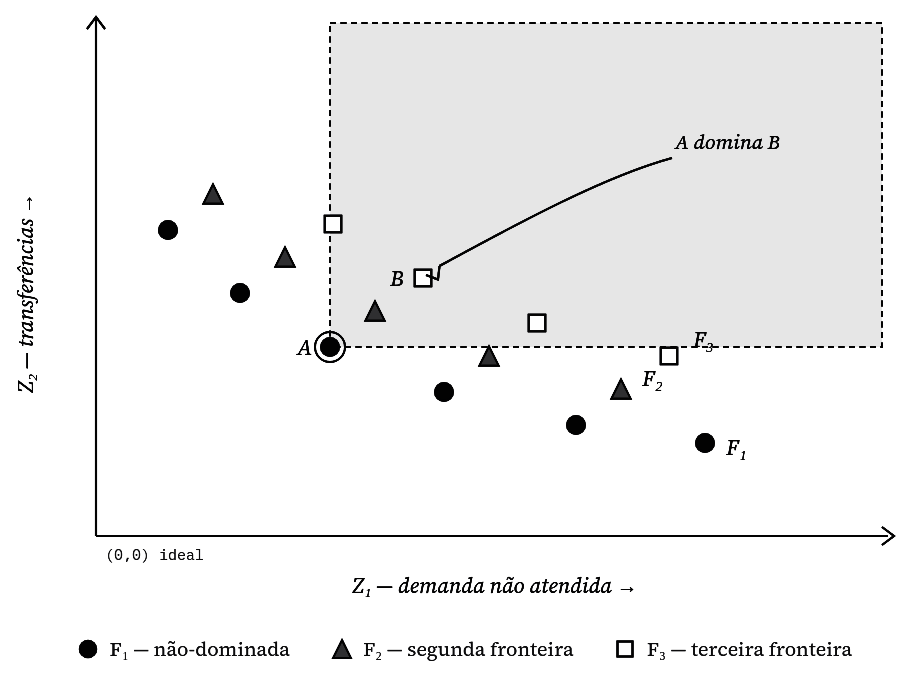
\includegraphics[width=\linewidth]{img/04_nsga-02_ordenacao.png}
                \caption{Ordenação não-dominada.}
                \label{fig:nsga-ord}
            \end{figure}
        \end{column}
    \end{columns}
\end{frame}

%%% Frame 4.4 — operadores customizados
\begin{frame}{Operadores customizados}
    \begin{columns}[c]
        \begin{column}{0.33\textwidth}
            \begin{figure}
                \centering
                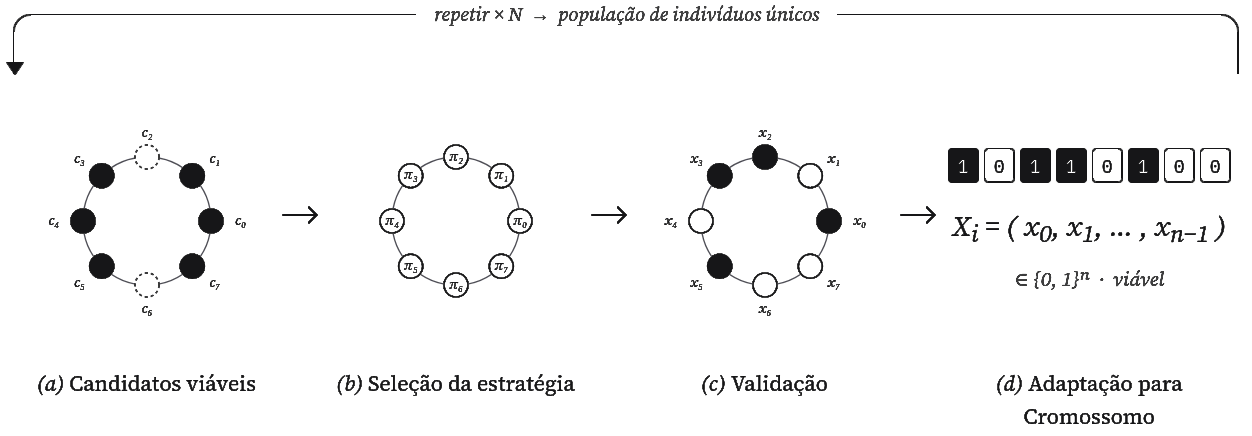
\includegraphics[width=\linewidth]{img/01_sampling.png}
                \caption{\footnotesize Amostragem com consciência de restrições.}
            \end{figure}
        \end{column}
        \begin{column}{0.33\textwidth}
            \begin{figure}
                \centering
                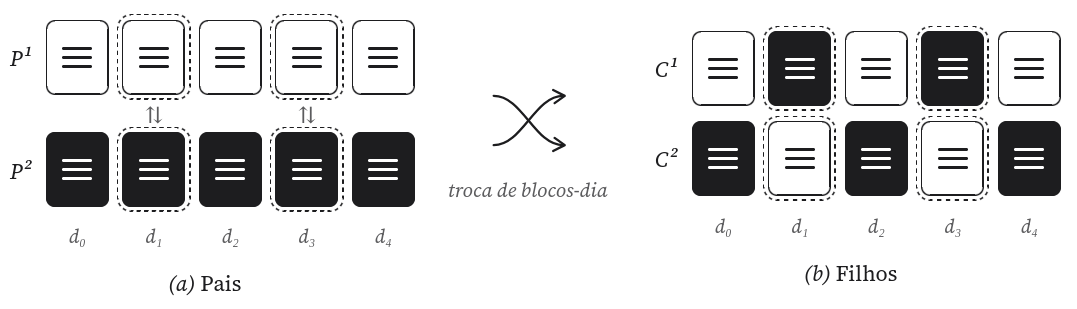
\includegraphics[width=\linewidth]{img/02_crossover.png}
                \caption{\footnotesize Cruzamento por blocos diários.}
            \end{figure}
        \end{column}
        \begin{column}{0.33\textwidth}
            \begin{figure}
                \centering
                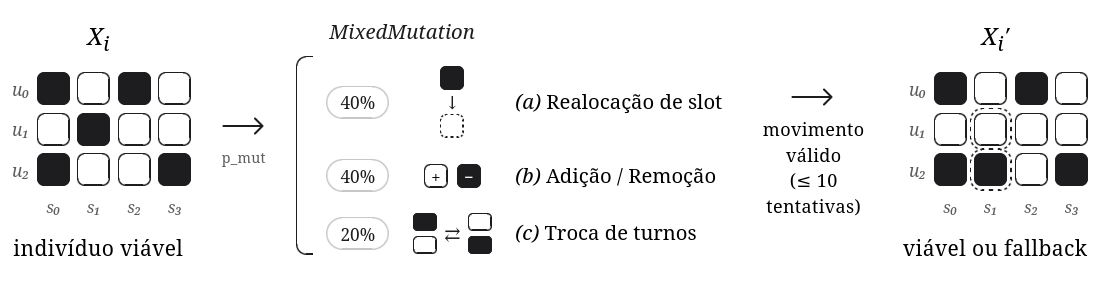
\includegraphics[width=\linewidth]{img/03_mutacao.png}
                \caption{\footnotesize Mutação por realocação de \textit{slot}.}
            \end{figure}
        \end{column}
    \end{columns}
    % TODO: operadores preservam coerência temporal da agenda; reduzem inviabilidade.
\end{frame}

%%% Frame 4.5 — Estendido vs Compacto (encoding)
\begin{frame}{Variantes: Estendido \emph{vs.} Compacto}
    \begin{figure}
        \centering
        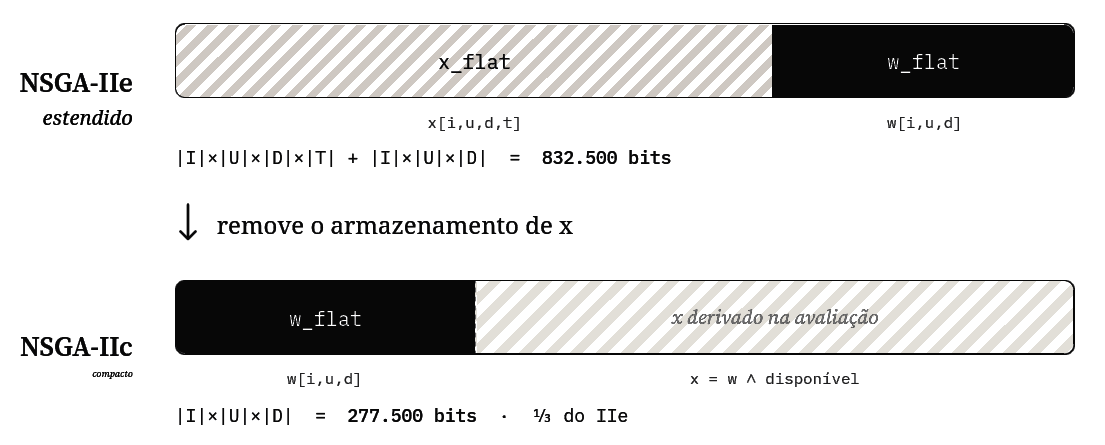
\includegraphics[width=0.82\linewidth]{img/05_encoding.png}
        \caption{Comparação dos \textit{encoders} NSGA-II Estendido e Compacto.}
        \label{fig:encoding}
    \end{figure}
    \begin{block}{}
        \begin{itemize}
            \item \textbf{Estendido:} cromossomo binário $x_{iudt}$ e $w_{iud}$ (alta dimensionalidade).
            \item \textbf{Compacto:} gene por par médico--dia ($\approx w$) $\rightarrow$ redução de $\sim$70$\times$ e mais gerações.
        \end{itemize}
    \end{block}
\end{frame}
